\section{No finite basis}\label{sec:no-basis}

A finite equational basis axiomatizes game equivalence: every valid equation follows from finitely many by substituting and replacing equals, as the laws of Boolean algebra do for classical connectives. With two players there is one, since the algebra is Kleene's three-valued logic (\cref{sec:discussion}). Reset and its one-owner expansion have finite bases, and hard equations do not prevent one. The fragment $\{\star_a,\cup\}$ is coNP-complete (\cref{thm:raw-pairs}), yet it has exactly the identities of meet-distributive bisemilattices \cite{HardingRomanowska2017}: the three semilattice laws for each operation and the distributive law
\[
 x\ow a(y\cup z)=(x\ow a y)\cup(x\ow a z)
\]
form a seven-equation basis (\cref{core:prop:choice-union-basis}). Owned choice thus distributes over union, though not over another player's choice (\cref{sec:rational}). So complexity does not explain the following failure: the owned choices of all roles together have no finite basis, even with winner constants and internal renaming.

\begin{theorem}[No finite basis]\label{core:thm:no-basis}
For every $K\geq3$, none of $\mathbf C$, $\mathbf A$, and $\mathbf A^{\rm sym}$ has a finite equational basis. For each of these signatures and every $n$, there is a finite algebra satisfying every identity of its winner algebra in at most $n$ variables but not all of them.
\end{theorem}

So no bound on the number of variables suffices, even with infinitely many laws.

\begin{figure}[htb]
\centering
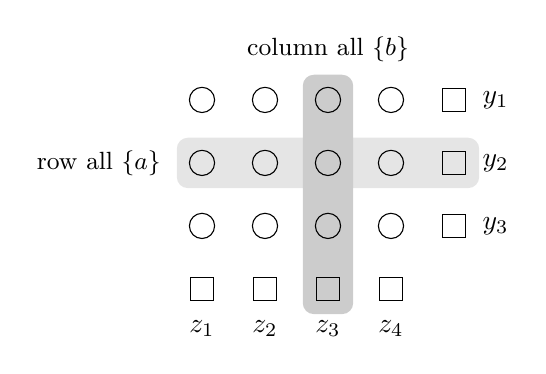
\begin{tikzpicture}[x=8mm,y=8mm,
  cell/.style={circle,draw,inner sep=0pt,minimum size=3.2mm},
  extra/.style={rectangle,draw,inner sep=0pt,minimum size=3mm}]
 \fill[black!10,rounded corners] (0.6,1.6) rectangle (5.4,2.4);
 \fill[black!20,rounded corners] (2.6,-0.4) rectangle (3.4,3.4);
 \foreach \i in {1,2,3} {
   \foreach \j in {1,...,4} \node[cell] at (\j,4-\i) {};
   \node[extra] at (5,4-\i) {};
   \node[anchor=west] at (5.3,4-\i) {$y_{\i}$};
 }
 \foreach \j in {1,...,4} {
   \node[extra] at (\j,0) {};
   \node[anchor=north] at (\j,-0.35) {$z_{\j}$};
 }
 \node[anchor=east,font=\small] at (0.5,2) {row all $\{a\}$};
 \node[anchor=south,font=\small] at (3,3.45) {column all $\{b\}$};
\end{tikzpicture}
\caption{The grid identity of \cref{core:thm:no-basis}, with the cells $x_{ij}$ drawn as circles. Each row with its $y_i$, and each column with its $z_j$, is combined by $\star_c$; $T$ combines the rows by $\star_a$, and $S$ the columns by $\star_b$. $T=\{a\}$ needs a row that is entirely $\{a\}$, and $S=\{b\}$ a column that is entirely $\{b\}$, but every row and column share a cell.}
\label{fig:grid}
\end{figure}

\begin{idea}
Arrange variables $x_{ij}$ in an $r\times s$ grid (\cref{fig:grid}), with an extra variable $y_i$ for each row and $z_j$ for each column. Let $T$ combine the rows by $\star_a$, after combining each row and its extra variable by $\star_c$, and let $S$ combine the columns in the same way by $\star_b$. Then $T=\{a\}$ only if some row is entirely $\{a\}$, and $S=\{b\}$ only if some column is entirely $\{b\}$. A row and a column share a cell, so these cannot both happen. Since $u\star_a T$ contains $u$ unless $T=\{a\}$,
\[
 u\subseteq(u\star_a T)\cup(u\star_b S),
\]
an identity in $(r+1)(s+1)$ variables, whose failure only the whole grid can detect. For each $n$, the countermodel is an algebra in which $T$ and $S$ can both be atoms, while any $n$ of its elements generate a subalgebra that genuine player views represent. It lives in a product of player views, each coordinate making at most one of $T$ and $S$ an atom, and adds one new element that both arms absorb. Each element of it sees a row through one bit: whether it is the atom of $a$ where that row is tested. So $n$ generators see the rows through at most $2^n$ patterns, and once $r,s>2^n$, two rows look alike to the subalgebra they generate, as do two columns. This repetition lets that subalgebra be represented by player views (\cref{core:thm:core-nfb}).

With winner constants and internal renaming, one copy of the countermodel for each role permutation, together with an absorbing element, keeps the obstruction: by \cref{gen:thm:core}, a valid identity that avoids the absorber comes from one of $\mathbf C$ (\cref{app:full-signature}).
\end{idea}

Identifying all ambiguous values, as observers of unique winners do (\cref{game:prop:obs}), removes the obstruction: the quotient of $\mathbf C$ has a basis of $K^2+3K+4$ equations in at most three variables (\cref{core:thm:atomic-basis}). The quotient has a near-unanimity term, one that returns $x$ whenever all its arguments but one equal $x$, and a finite algebra with such a term has a finite basis \cite{Baker1977}. The core has none, since on ambiguous inputs every core term is the union of its variables, so this route to a basis is closed for $\mathbf C$.
